\documentclass[tikz]{standalone}
\usepackage{amsmath}
\usepackage{mathtools}
\usepackage{helvet}
\usepackage[T1]{sansmath}
\usetikzlibrary{arrows,decorations.markings}
\renewcommand{\familydefault}{\sfdefault}
\normalfont

\begin{document}
\begin{sansmath}

\tikzstyle{circ} = [circle,draw,thick,fill=blue!10,minimum size = 1cm,thick]
    
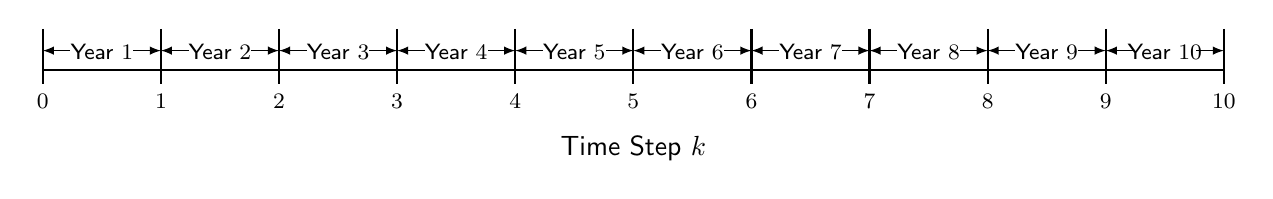
\begin{tikzpicture}[auto]
    %\draw[help lines] (0,2) grid (15,-2);
    
    \node (xlabel) at (7.5,-1) {Time Step $k$};
    
    \draw [thick] (0,0)--(10*1.5,0);
    \foreach \k in {0,...,10}
    	\draw [shift={(1.5*\k,0)},thick] (0pt,15pt)--(0pt,-5pt) node[below] {\footnotesize $\k$};
    \foreach \k in {1,...,10}{
    	\draw [thick] (1.5*\k-0.75,0) node[above] {\footnotesize Year $\k$};
    	\draw [latex-] (1.5*\k-1.5,0.25) --++ (10pt,0);
    	\draw [latex-] (1.5*\k,0.25) --++ (-10pt,0);
    }
    	
\end{tikzpicture}

\end{sansmath}
\end{document}
